\documentclass[preprint]{sigplanconf}
%\documentclass[12pt]{article}

\usepackage[colorlinks=true]{hyperref}
\usepackage{amsmath,amssymb} 
\usepackage{fancyvrb}

%\newenvironment{template}{\sffamily}

\usepackage{graphics,epsfig}

\newcommand{\tens}[1]{\mathbf{#1}}

%\title{Network Tensor Contraction Engine: Project Demo Requirements Document}
%\author{David M. Rogers and James Horton}

%\title{ A High-Level Language for Basic Tensor Linear Algebra}
\begin{document}

\title{ Efficient Primitives for Standard Tensor Linear Algebra}
\authorinfo{David M. Rogers}
{Department of Chemistry, \\
University of South Florida, \\
Tampa, Florida.}
{Email: davidrogers@usf.edu}

\maketitle

\begin{abstract}
  This paper presents the design and implementation of low-level
library to compute general sums and products over multi-dimensional arrays (tensors).
Using only 3 low-level functions, the API at once generalizes
core BLAS1-3 as well as eliminates the need for most tensor transpositions.
Despite their relatively low operation count, we show that these transposition steps
are actually performance limiting in most typical use cases for BLAS on tensors.
The execution of the present API achieves peak performance on the same
order of magnitude as for vendor-optimized GEMM
by utilizing a code generator to output CUDA source code for all computational kernels.
The outline for these kernels is a multi-dimensional generalization
of the MAGMA BLAS matrix multiplication on GPUs.  Separate
transpositions steps can be skipped because each kernel allows arbitrary
multi-dimensional transpositions of the arguments.
The library, including its methodology and programming techniques, are
made available in SLACK.  Future improvements to the library include
a high-level interface to translate directly from a \LaTeX{}-like equation
syntax to a data-parallel computation.
\end{abstract}

\section{ Introduction and Background}

  Linear algebra on large arrays is central to scientific computing and all applied mathematical
modeling.  An increasingly large number of problem structures, however,
do not fit well to the simple vector-or-matrix model presented by basic linear
algebra subprograms (BLAS)\cite{blas} -- which form the currently accepted foundation for all
dense matrix operations.  Instead, most dense numerical algorithms fit much more naturally
to arrays -- a logical generalization including vectors (dimension 1) and matrices (dimension 2)
as special cases.  Their popularity can be easily seen by the thousands of packages based
on the general array implementation in python's {\em numpy} package.\cite{numpy}

  An $n$-dimensional array is defined as a block of data with $n$ indices, $i_0, \ldots, i_{n-1}$.
Each index has a contiguous range, $i_k = 0,\ldots,s_k-1$, where $s = \{s_0,\ldots,s_{n-1}\}$
is the shape of the array.  The set of all arrays of shape $s$ is denoted $\mathcal T_s$ (the terms
tensor and array are used interchangeably).
Here, we assume dense, non-symmetric arrays, which require memory space for
$\Pi_{k=0}^{n-1} s_k$ unique array elements.

  Despite their popularity, there are no general alternatives to BLAS operations for multidimensional
arrays.  At a minimum, these operations should allow addition, multiplication, contraction,
and transposition of arrays.  The {\em numpy} implementation also provides
several (map-like) per-element functions such as sine, cosine, and absolute values,
as well as (reduce-like) single-index operations such as min/max/sum.
Currently, {\em numpy}'s low-level implementation of these operations relies on a general
tensor transposition implemented on the CPU combined with a translation to BLAS.
It does not permit high-level abstraction or heterogeneous execution.

  Standard linear array computational kernels (SLACK) is intended to be a functional
replacement for BLAS that works efficiently with arrays.
Source code created in the course of the present work has been
made available in an open-souce library (USF-SLACK) that implements
this interface.  One major result of this work has been to demonstrate
that these kernels can be just as efficient as current high-performance
BLAS implementations.

  Several works have addressed the issue of generating code to efficiently
compute tensor operations in parallel.%  As already noted, the MAGMA library
%uses a code generation strategy that shares .
%Our implementation is based on MAGMA's stencil for matrix multiplication
%on GPUs.\cite{}
  The tensor contraction engine (TCE) translates
a domain-specific language for tensor contractions occurring in the field of
chemistry into a series of low-level FORTRAN loops for tensor
summations and transpositions.\cite{tce}  Much of the development effort for that
code has gone into identifying high-level reorganizations of sets of tensor operations,
and work is still underway to improve parallel execution methods.
The cyclops tensor framework (CTF)\cite{ctf} is a similar project aimed at
implementing efficient tensor contractions for large tensors stored
in distributed global memory.  Its interface uses essentially equivalent {\tt contract} and {\tt sum}
functions, but specifies permutations by labeling all indices on each input tensor
using character strings and outputs to $B$ instead of $A$.
One of the motivations for the present work is the observation stemming from these projects
that tensor transposition accounts for nearly half the execution time of typical problems.\cite{spaghetty}
Similar observations have motivated development on the tensor contraction generator (TCG),
another low-level CUDA code generator for tensor contractions.\cite{tcg,wma11}
Unfortunately, performance results for TCG were only reported for double precision
(shown to achieve a peak of around 40 Gflops), but not compared to vendor-optimized GPU
BLAS kernels.  In addition, the lack of a straightforward syntax for specifying contractions
made TCG less accessible.
Redesigning the syntax of these operations both eliminates
this additional cost as well as divorces the algorithm from its domain-specific context.

  A few researchers have considered simply finding optimal methods for
translating of tensor contractions to standard BLAS calls.\cite{slice}
At a best, these translations are still subject to the
cost of tensor transpositions.  In the worst case, the translation requires multiple
level-1 BLAS operations with sparse data accesses that cannot be made cache-efficient
and thereby slow execution times.

  Rather than pursuing this strategy, the present work adopts an identical
outline to the tunable matrix multiplication kernel in the Matrix algebra on
GPU and multicore architectures (MAGMA) library,\cite{magma}
but adds awareness for multi-index input and output tensors.  The result
is an identical computation for each tile of the output matrix, and only required
modified read and write loops for accessing those tile locations.

  Section~\ref{s:low} of this paper presents a low-level API comprised of only three basic operations,
-- {\tt tscale}, {\tt tadd}, and {\tt tdot}.  These  cover all basic addition, multiplication, transposition,
and contraction operations (Table~\ref{t:blas}).
They are therefore a generalization of the core of BLAS levels 1-3
-- excluding routines involving packed storage, symmetry, $L_1$ norms, or specialized rotation functions.
Section~\ref{s:gen} outlines the operation of the code generator which
achieves high performance kernels by automatically generating implementation code for
arbitrary thread block and output tile sizes.
Section~\ref{s:high} presents the high-level organization used to automatically execute a
set of tensor algebra operations in parallel, including automatically
managing intermediate values.

  A performance study is presented in Sec.~\ref{s:perf}.  Without optimizing the tile-sizes
or using texture mapping, the kernels corresponding to SGEMM are about half as fast
as the performance-tuned MAGMA library.  Significantly, these speeds are maintained
for multi-index tensor products, where they hold a significant advantage over a na\"{\i}ve
BLAS-based implementation strategy.
It is shown that emulating those tensor products by
DGEMM sandwiched between tensor transpositions decreases overall performance by up
to a factor of 100.%  Finally, near-linear scaling is shown for compound tensor algebra
%expressions interpreted from \LaTeX{} code.

\section{ Low-level Contraction Operations}\label{s:low}

  The two routines, {\tt tadd} and {\tt tdot}, cover all addition, multiplication, transposition,
and contraction operations.  The additional routine, {\tt tscale}, is the equivalent of BLAS' \_SCAL,
and is included for completeness.
The routine {\tt tadd} is a fused tensor transpose plus add.
Its inputs are two tensors of the same dimensionality, $A \in \mathcal T_{s_0,s_1,\ldots,s_{n-1}}$
and $B \in \mathcal T_{t_0,t_1,\ldots,t_{n-1}}$, along with an index permutation,
$\sigma$, mapping from indices of $B$ to indices of $A$.
The two tensors must have equivalent shapes under permutation, so $t_k = s_{\sigma(k)}$.

  For compact notation, we define super-indices as a complete tuple of indices,
$I = (i_0, i_1, \ldots, i_{n-1})$, and permutations of tuples as
$I = \sigma \circ J$, where $i_{\sigma(k)} = j_k$.
For numerical efficiency, two scaling factors are included in {\tt tadd}
inputs, and the result of the operation is stored in-place in the tensor $A$.
The combined operation is logically,
\begin{equation}
\text{\tt tadd} \quad A[I] := \alpha A[I] + \beta B[\sigma^{-1} \circ I]
\end{equation}

  The use of a permutation on the indices of $B$ is necessary to remove the need
for transpositions of input arguments.  The input matrix, $A$ is not transposed.
Its index order carries through to the output.  Necessary transposes can usually
be folded into the eventual function consuming the output of `{\tt tdot}'.  Nevertheless,
a matrix transpose as expressed by {\em numpy}'s {\tt transpose}($A, \sigma^{-1}$),
can be written as {\tt tbin}(`+', 0.0, Zero, 1.0, $A$, $\sigma$).  

  This obviously generalizes {\tt axpy}, which itself generalizes {\tt copy} and {\tt scal}.
In addition, changing the binary operation is comparatively much simpler from the end-user's
perspective when code is generated from a template.  This allows, for example,
building up direct products.

  Finally, the structure of `{\tt tadd}' can be relaxed to allow both reductions along
several indices of $B$ or introduction of new indices into $B$.  Both can be understood
as broadcasting operations\cite{numpy} involving an index of size $1$ from one
array and an index with an arbitrary size from the other.  Note that inserting an index of size 1
is only a logical operation, and does not change the memory layout of the array.
These only require accessing memory in $A$ and $B$ via strides, using
\begin{equation}
A[I] \Rightarrow A\left[\sum_{k=0}^{n-1} i_k \text{stride}_k\right].
\end{equation}

  The trick relies on the fact that moving along an index with stride 0
does not change the memory location accessed.
For a reduction, an index is inserted into $A$ with size 1 and stride 0.
Summation along the corresponding index in $B$, will accumulate into
to the same output location.
For a broadcast, the $B$ index has size 1, and stride 0.
The tensor $B$ will then appear to be copied along that dimension.

  Many other useful functions also follow the same basic pattern of {\tt tadd},
replacing `+' with any commutative operation on 2-arguments.
The direct product just replaces `+' with, `*'.  Reductions can usefully replace
`+' with `min' or `max', etc.

\subsection{ Tensor Contraction}

  The `{\tt tdot}' operation expresses a general tensor contraction.  Tensor
contractions are a special type of marginalization product function\cite{mpf} where
indices in $A \in \mathcal T_{s_0,\ldots,s_{n_A-1}}$ (and respectively $B_{t_0,\ldots,t_{n_B-1}}$)
are divided into two disjoint sets -- $n$ inner and $n_A - n$ (resp. $n_B-n$) outer indices.
The inner indices are to be summed over and must have sizes that
match between $A$ and $B$.  The outer indices are not constrained,
and are output to a third tensor, $C$.  This output tensor therefore has dimension
$n_C = n_A + n_B - 2 n$.

\begin{figure}
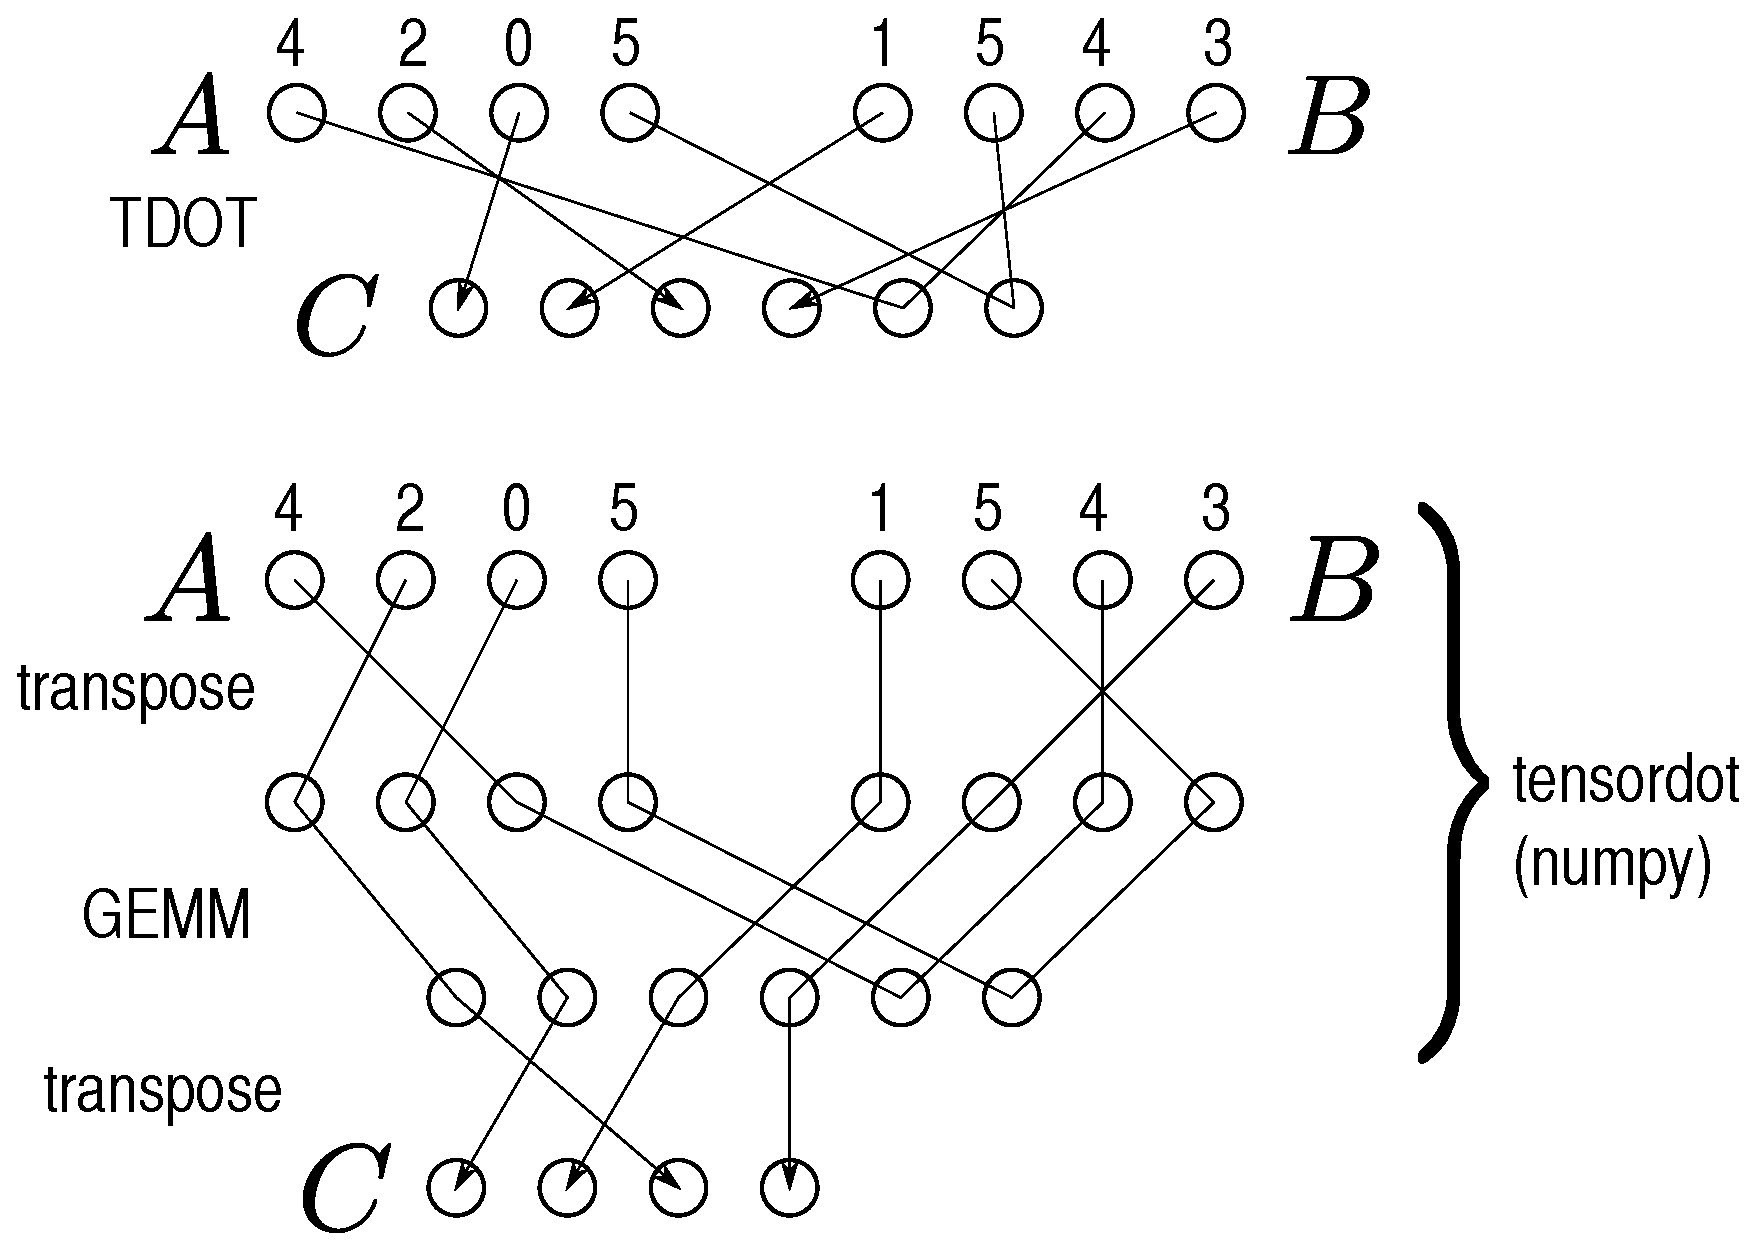
\includegraphics[width=0.45\textwidth]{contr.eps}
\caption{Role of index permutations in the tensor contraction.
Permutations of $A$ and $B$ indices specify both the order of the
contraction result, $C$, and an artificial ordering on the contracted indices.
For comparison, a common emulation using GEMM sandwiched between tensor
transpositions is shown below.}\label{f:contr}
\end{figure}

  We specify a generic tensor contraction using two permutations,
$\sigma_A$ and $\sigma_B$, mapping indices in A (resp. B), to indices in
an expanded, logical tensor, $C' \in \mathcal T_{u_0, \ldots, u_{n_C+n-1}}$.
The complete tensor contraction is a sum over the last $n$ indices of this expanded
tensor,
\begin{align}
\text{\tt{tdot}} \quad C[u_0,\ldots,u_{n_C-1}] &:= \alpha \sum_{u_{n_C}, \cdots, u_{n_C+n-1}} C'[u_0,\ldots,u_{n_C+n-1}]  \notag \\
 & + \beta C[u_0,\ldots,u_{n_C-1}] \\
 C'[u_0,\ldots,u_{n_C+n-1}] &= A[i_0,\ldots,i_{n_A-1}] B[j_0,\ldots,j_{n_B-1}]
\end{align}

  The expanded tensor is illustrated in Fig.~\ref{f:contr}.
The indices $\{u\}$ are such that $u_{\sigma_A(k)} = i_k$ and $u_{\sigma_B(k)} = j_k$.
The outer indices of $A$ ($B$) thus map uniquely to the left part of $C'$,
$\sigma_A(k) < n_C$ ($\sigma_B(l) < n_C$, with $\sigma_A(k) \ne \sigma_B(l)$),
while the inner indices go to the right in pairs, so $\sigma_A(k') \ge n_C$ ($\sigma_B(l') \ge n_C$,
with one equivalent map, $u_{m} = \sigma_A(k') = \sigma_B(l')$, for each $m \ge n_C$).

  The {\tt tdot} operation encompasses a large subset of BLAS 1-3.  Table~\ref{t:blas} lists several
translations.
\begin{table*}
\begin{tabular}{lll}
$x \gets \alpha x$ & \_SCAL(N,$\alpha$,X) %\\
    & tscale($\alpha$, X, N) \\
$y \gets x$ & \_COPY(N,X,Y) %\\
    & tadd(0.0, Y, (N), 1.0, X, (N), (0)) \\
$y \gets \alpha x + y$ & \_AXPY(N,$\alpha$,X,Y) %\\
    & tadd(1.0, Y, (N), $\alpha$, X, (N), (0)) \\
r $\gets x^T y$ & \_DOT(N,X,Y) %\\
    & tdot(0.0, R, 1, 1.0, X, (1,N), (0,1), Y, (N), (1)) \\
$y \gets \alpha A x + \beta y$ & \_GEMV(`T', M, N, $\alpha$, A, X, $\beta$, Y) %\\
    & tdot($\beta$, Y, 1, $\alpha$, A, (N, M), (0,1), X, (M), (1)) \\
$y \gets \alpha A^T x + \beta y$ & \_GEMV(`N', M, N, $\alpha$, A, X, $\beta$, Y) %\\
    & tdot($\beta$, Y, 1, $\alpha$, A, (N, M), (1,0), X, (N), (1)) \\
$A \gets \alpha x y^T + A$ & \_GER(M, N, $\alpha$, Y, X, A) %\\
    & tdot(1.0, A, 2, $\alpha$, X, (N, 1), (0,2), Y, (M, 1), (1,2)) \\
$C \gets \alpha A B + \beta C$ & \_GEMM(`N', `N', M, N, K, $\alpha$, B, A, $\beta$, C) %\\
    & tdot($\beta$, C, 2, $\alpha$, A, (N,K), (0,2), B, (K,M), (2,1)) \\
$C \gets \alpha A^T B + \beta C$ & \_GEMM(`N', `T', M, N, K, $\alpha$, B, A, $\beta$, C) %\\
    & tdot($\beta$, C, 2, $\alpha$, A, (K,N), (2,0), B, (K,M), (2,1)) \\
$C \gets \alpha A B^T + \beta C$ & \_GEMM(`T', `N', M, N, K, $\alpha$, B, A, $\beta$, C) %\\
    & tdot($\beta$, C, 2, $\alpha$, A, (N,K), (0,2), B, (M,K), (1,2)) \\
$C \gets \alpha A^T B^T + \beta C$ & \_GEMM(`T', `T', M, N, K, $\alpha$, B, A, $\beta$, C) %\\
    & tdot($\beta$, C, 2, $\alpha$, A, (K,N), (2,0), B, (M,K), (1,2)) \\
\end{tabular}
\caption{Translation from C, row-major shorthand notation to legacy BLAS and
to {\tt tadd} / {\tt tdot} for arrays of dimension 1 and 2.  All lower dimensions (IDX, etc.) are 1.
Argument order for {\tt tadd} is $\alpha$, A, A shape, B, B shape, B permutation.
Argument order for {\tt tdot} is  $\beta$, C, dimension of C, $\alpha$, A, A shape, A permutation, B, B shape, B permutation.  Note that {\tt tdot} is symmetric to interchanging $A$ and $B$.}\label{t:blas}
\end{table*}

  A straightforward implementation of tensor contraction is provided {\tt tensordot} in the {\em numpy} library
with a fixed ordering of all outer indices.\cite{numpy}
First the tensors $A$ and $B$ are transposed to $A'$, $B'$,
so that the inner indices of both are moved to the right-hand side in matching order.
The outer indices are left in their input ordering.  Because they are contiguous, all outer indices
can now be addressed using a single, combined index, and similarly for the inner indices.
The tensor product then reduces to a matrix product, $A' B'^T$.
To emulate the present definition of contraction, this end result needs to be supplemented
by a final transpose to re-order the output indices.  The efficiency of this method is compared to the
direct kernel versions in Sec.~\ref{s:perf}.

\section{ Code Generation Strategy}\label{s:gen}

  The low-level kernel execution for {\tt tdot} is essentially a GEMM, but
has the added difficulty of dealing with arbitrary numbers of indices.
The most simplistic implementation is to combine all $n_C$ output indices
of $C$ into one omnibus dimension, and all $n$ inner indices
into another.  Each iteration of a double-loop decodes the corresponding
locations in $A$, $B$, and $C$.  The timings for this implementation, using
1 CUDA thread per output location are almost equivalent to the transpose-sandwiched
version.

  A much better performance is achieved by adopting the MAGMA library
strategy of loop nesting.\cite{magma}  There, a $T_A \times T_B$ block of threads each
compute $W_A \times W_B$ output locations to produce an $T_A W_A \times T_B W_B$
output tile of $C$ for each thread block.  Each thread sums over the whole contracted
dimension, $K$.  This strategy decreases the cost of memory movement by relying on the
hardware to combine reads from all threads into sequential accesses of CUDA global memory.
Both copies from $A$ and $B$ as well
as computation of the output tile are parallelized among the thread block.

  We have adapted this strategy to {\tt tdot} by defining the output tile
to be composed of 2 omnibus dimensions -- all output indices from $A$
and all output indices from $B$.  The thread and work blocks are therefore sub-divided as
$T_A = \{T^A_k | \sigma_A(k) < n_C\}$, and similarly for $T_B$, $W_A$, and $W_B$.
The code generator works for fixed tensor dimensions and permutations, so that
the index decoding steps are explicit instead of loops over arbitrary number of dimensions.
Copies in the nested inner loops have known sizes, and are written out explicitly
using simultaneous access to $A$ and $B$ that can be coalesced by the hardware.

  Although the output tile is logically indexed by output dimensions of
$A$ and then $B$ (as for the output of {\tt tensordot} -- Fig.~\ref{f:contr}),
the actual output is done directly to the correct locations in $C$.
This only requires putting the strided access in the right place.
It has a large practical advantage in that the physical
memory is only accessed once.

\section{ Performance Results}\label{s:perf}

  This section presents timing results for single-precision {\tt tdot} operations computed
on an NVIDIA GTX980 (1.38 GHz, 4 GB memory) with NVIDIA proprietary
kernel driver version 346.72 for Ubuntu server 14.10 compiled with nvcc 7.0.27.  Reported timings
are the fastest out of 10 trials and do not include CPU to GPU transfer times.
This GPU is one of the first releases to use the new Maxwell redesign of
the K20.  Because it has been designed for consumer graphics,
there are fewer double-precision floating point units per stream processor.
MAGMA timings for DGEMM on this GPU peaked around 150 Gflops, while those
for SGEMM were significantly higher at 4000 Gflops.  Because of this limitation,
only single precision timings are reported below.

  Fig.~\ref{f:gflops} compares alternative methods for computing the 4-index
tensor contraction illustrated in Fig.~\ref{f:contr}.  The horizontal
axis shows $N$, the size of each dimension for the case where all shapes are
$\{N,N,N,N\}$ hypercubes.
The upper panel shows throughput for the SGEMM kernel on matrices of size $N^2 \times N^2$.
The right side of Fig.~\ref{f:contr} shows how the central step
of the contraction is essentially a matrix multiplication.  The test kernel
computes one output element of the matrix per thread, and has fairly
constant performance around 10 Gflops.
The optimized MAGMA 1.6.1 kernel and cuBLAS performance is significantly
higher, peaking around 3000 - 4000 Gflops.  MAGMA uses a 16$\times$16 thread
block to compute 36 output elements each -- for an output tile size of 96$\times$96.
cuBLAS shows variable performance, likely the result of a larger tile size.

  Notably, Fig.~\ref{f:gflops} shows that {\tt tdot} achieves performance on the same order
of magnitude as state of the art optimized BLAS routines.
Using the same tile sizes as MAGMA (16$\times$16 thread block and 96$\times$96 output tile)
for the generated {\tt tdot} kernel gives around 2500 Gflops compared to MAGMA's 3500.
Because the basic outline of the kernel is identical between MAGMA and
{\tt tdot}, the lower performance can be attributed to
minor differences in the layout and orderings of copies between global memory,
shared memory, and registers.

\begin{figure}
{ \centering
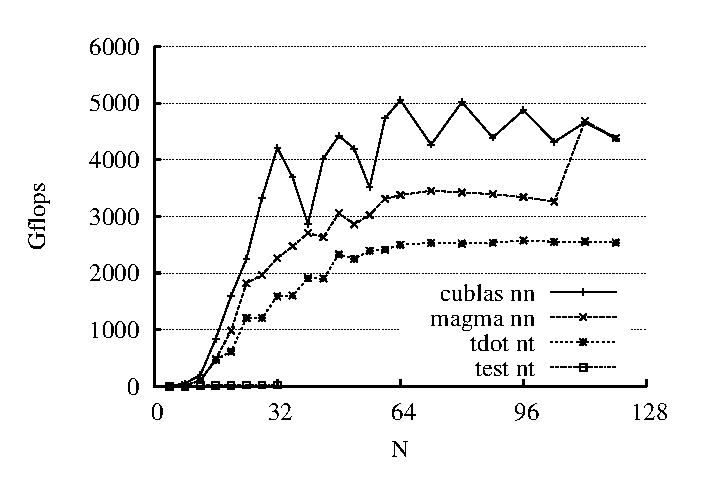
\includegraphics[width=0.45\textwidth]{sgemm.eps}
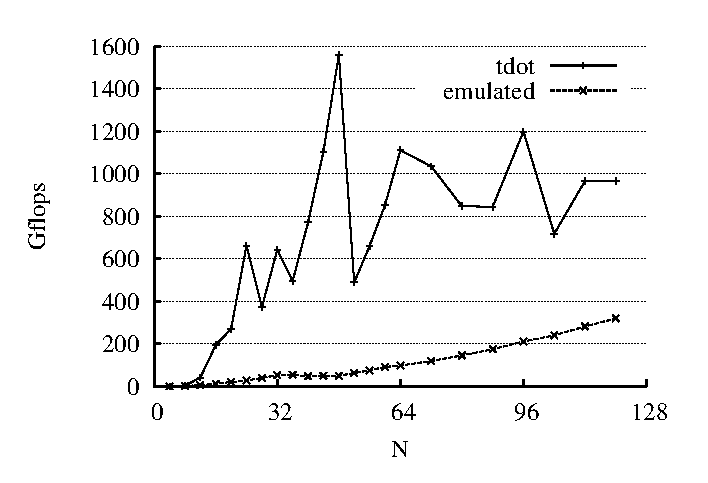
\includegraphics[width=0.45\textwidth]{gflops.eps} }
\caption{Performance comparison between MAGMA and generated contraction
kernel, {\tt tdot}.  The upper panel compares the fastest versions of the SGEMM kernel,
which happened to be NN for MAGMA and NT for {\tt tdot}.  The lower panel
shows that including transposes greatly decreases overall throughput for emulating {\tt tdot},
while a direct 4-index {\tt tdot} kernel performs at about half the speed of {\tt tdot} for SGEMM.}\label{f:gflops}
\end{figure}

  The lower panel of Fig.~\ref{f:gflops} compares the overall performance for the full
4-index contraction of Fig.~\ref{f:contr} using a {\tt tdot} kernel created
to directly compute the contraction against an emulation strategy using
SGEMM sandwiched between transposes.  The emulated timings are computed
by adding the timings for transposing both inputs, performing SGEMM using the MAGMA library,
and transposing the final output.  Even though the matrix multiplication
step scales as $O(N^6)$, while transposition scales as $O(N^4)$,
the matrix transpositions severely limit the overall throughput.  It should be noted
that tensor sizes larger than N = 128 could not be tested as they exceed the 4GB memory
limit of the device.

  Fig.~\ref{f:pct} provides further detail on the time spent during tensor transposition
{\em vs} computing matrix multiplication.  The transpositions occupy a significant
fraction of time for all sizes.  In fact, for most reasonable tensor sizes, the transposes
occupy more than 90\% of the time.  The requirement for separate transpositions
explains the low overall throughput for emulating a direct tensor contraction.

\begin{figure}
{ \centering
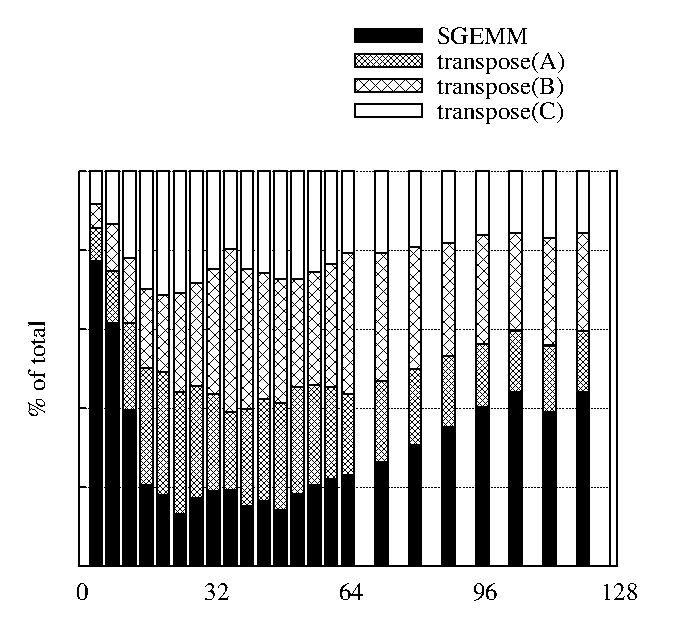
\includegraphics[width=0.45\textwidth]{pct.eps} }
\caption{Breakdown of time spent in emulated {\tt tdot} for Fig.~\ref{f:contr}.
Host $\leftrightarrow$ device memory transfer time is not included.
SGEMM timings are copied from MAGMA's timings on an $N^2 \times N^2$ matrix.
Transpose timings count only the transposes that would be done during {\tt tensordot}
within the {\em numpy} library (not including python overhead).
Even for large tensors, a majority of the time is spent in CPU transpose.}\label{f:pct}
\end{figure}
  
\section{ Conclusions and Future Work}

  We have shown that computing tensor transpositions can be a significant
bottleneck to general tensor algebra.  Legacy BLAS routines do not provide
a means to cope with this issue.  Instead, we propose a simple and
general API for combining transpositions into tensor contractions and summations.
This provides a means to hide the cost of tensor transpositions
inside the data access already performed during the normal course of tensor multiplication.
We have shown a preliminary implementation of this API that provides
speed comparable to high-performance BLAS.

  Many factors influence the efficiency of {\tt tdot} kernels.  These include
both the shape of the tensors $A$, $B$, and $C$ relative to the thread
and work block shape as well as the index permutations applied to $A$ and $B$.
In all cases, it is reasonable to expect the largest performance improvements
when $A$, $B$, and $C$ are all accessed sequentially within each tile.
This is easily achieved when the multi-dimensional tile size contains large work segments
in locations corresponding to the last (sequential) indices of $A$, $B$, and $C$.
By working on a block at a time, loop nesting also helps minimize the cost of performing
transpositions.

  Tensors present unique challenges in that high-dimensional tensors
have many indices with small shapes.  The performance data in Fig.~\ref{f:gflops}
shows non-uniform behavior partly because each dimension has to be expanded
to the nearest output tile-size.  Especially for small dimensions,
this padding can be very costly because it is multiplied by the
sizes of all other dimensions.

  This case of a few small dimensions is precisely where code generation
is most useful.  When they occur in the first few indices, generation can remove
the need for padding the input tensor.  If these small dimensions occur in the tensor's
last few indices, generated code can still create sequential loads, since memory
can be copied to registers in input tensor order, but written in output tensor order.
Non-sequential access then occurs only occurs on sub-blocks stored in device registers.

  Future work should be invested in finding more general ways to optimize the layout and access patterns
of nested sub-blocks.  It would be interesting to pursue a strategy connecting
a high-level code to the low-level just-in-time compilation to CUDA hardware with
new compute capability.  Major productivity gains for end-users can also be gained by providing
even higher-level interfaces to run sets of {\tt tdot} and {\tt tadd} operations on multiple input and
output tensors.  A separate paper describes the implementation of a DAG scheduler
for tensor operations in the SLACK library.

\bibliographystyle{unsrt}
\bibliography{lit}

\end{document}


\section{ Introduction}

  Nevertheless, the high-level organization
chosen for the present project is a departure from the organization of the high-level
routines in the MAGMA library.  Here, we have chosen to use a strict functional
syntax tree, as opposed to that library's use of a series of imperative routines written
using high-level aliases for tuned low-level codes.  The imperative style allows greater
control over the synchronization and memory management during
intermediate steps in the computation.  In principle this allows hand-tuning to
achieve the highest possible performance.  The functional programming style
adopted here acknowledges that in practice these low-level details are very
difficult to anticipate, and that it is impossibly time-consuming to hand-tune every
high-level function.  Instead, SLACK expresses all compound operations using an abstract
syntax tree, which is executed using a generic parallel scheduling back-end.
Optimizations are expected to be implemented through syntax
tree transformations.

  The Theano project\cite{theano} has a similar perspective.  It builds a directed acyclic graph
representation of a series of tensor operations in order to gain run-time-efficiency
by simplification on that representation.  Another noteworthy python
library using functional representations to generate code is the FEniCS project.\cite{fenics}
That project implements a domain-specific language for partial differential
equations on finite element meshes from which C++ code is generated.

  The tensor contraction engine (TCE) translates
a domain-specific language for tensor contractions occurring in the field of
chemistry into a series of matrix BLAS operations and low-level code for transpositions.\cite{tce}
It also produces the equations in \LaTeX{} form as a by-product.
Distinct from this work, TCE, along with a related engine, \cite{ctf}, make use of
statically planned distributed-memory array storage and execution.
One of the motivations for the present work is the observation that tensor transposition accounts for
nearly half the execution time of typical problems.  Redesigning the high-level
syntax of these operations both eliminates this additional cost as well as
divorces the algorithm from its domain-specific context.

\section{ Functional Interface}\label{s:high}

  The SLACK library expresses a series of tensor operations using a
directed acyclic graph (DAG).  Nodes in the DAG correspond
to intermediate results, while arrows show data dependencies.  The leaves
of the tree are input tensors, and the root represents
the final output result.  Internally, each DAG node is represented as an
operation and a list of dependencies.

\begin{figure}
{\centering
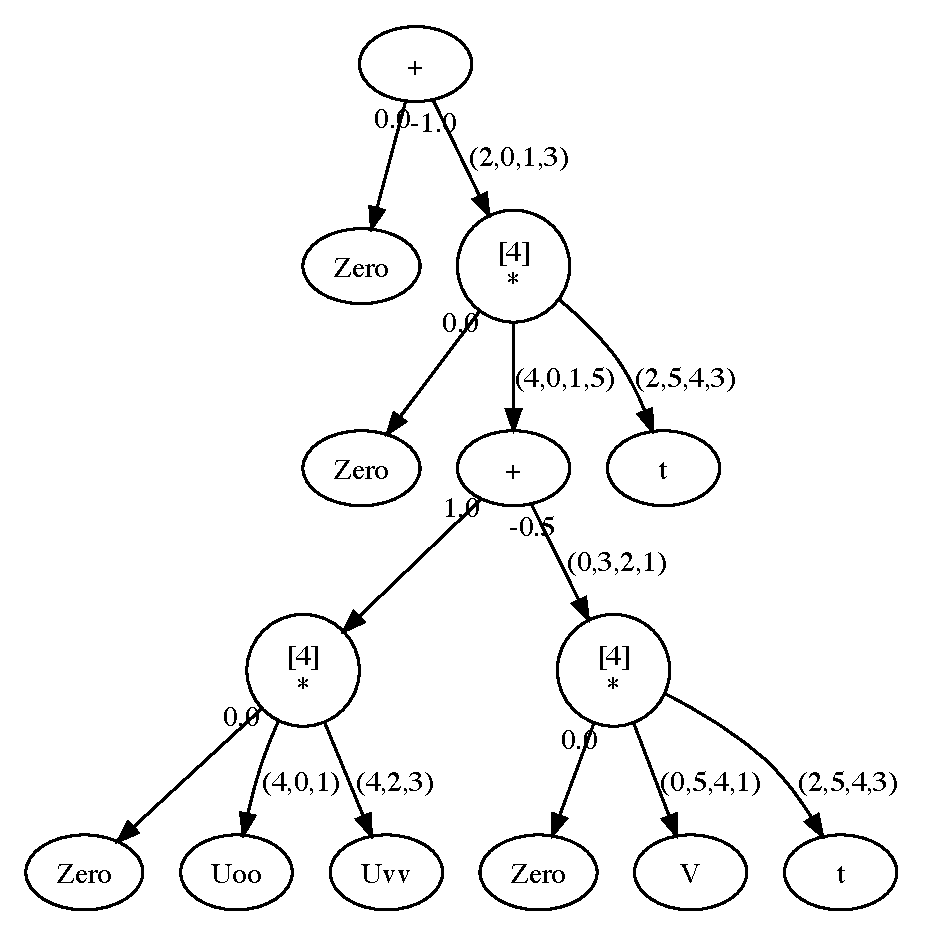
\includegraphics[width=0.45\textwidth]{Cstart.eps}
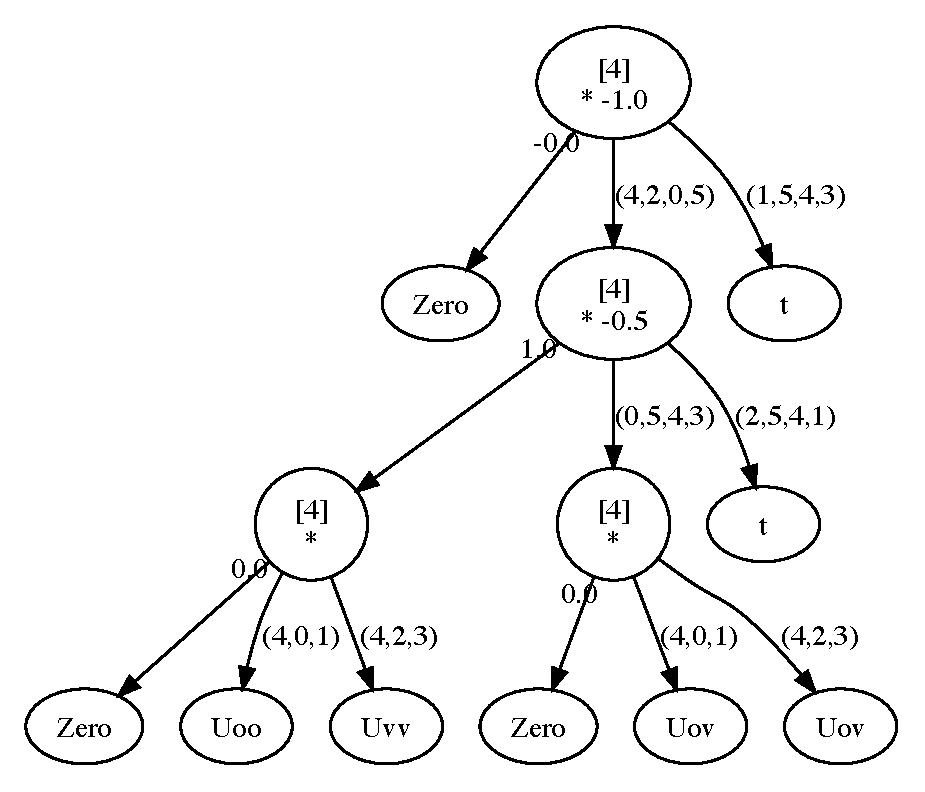
\includegraphics[width=0.45\textwidth]{C.eps}}
\caption{Initial (left) and simplified (right) expression trees parsed from \LaTeX{} source for Eq.~\ref{e:C}.  Execution order is from bottom to top, with the topmost node representing the output, $C$.  Index symbols have been converted to permutations, $\sigma$, shown near the end of each arrow. Contractions are labeled with
$* \alpha$ and the dimension of the output tensor in brackets.  Scales ($\alpha$ / $\beta$) are shown at the tops of arrows where applicable.  The topmost 4-index contraction forms
the example shown in Fig.~\ref{f:contr}.}
\label{f:dag}
\end{figure}

  Figure~\ref{f:dag} shows the initial and final DAGs resulting from
parsing the mathematical expression,
\begin{equation}
C^{ab}_{ij} = -\sum_{kc} \left(
                        \sum_Q \text{Uoo}^Q_{ki} \text{Uvv}^Q_{ac}
                        - 0.5 \sum_{ld} V_{kdlc} t^{ad}_{li}
                                     \right) t^{bc}_{kj}  \label{e:C}
\end{equation}
During (bottom-up) parsing, permutations are generated by maintaining an ordered list of `active' indices
(as well as scaling factors) at each stage during the parse.  At the end of the parse, a final tensor transpose
is added to convert these active indices to the desired output order.
Superscripts are put before subscripts.
So, for example, $\sum_Q \text{Uoo}^Q_{ki} \text{Uvv}^Q_{ac}$
has order $[kiac]$, and its contraction with $t^{bc}_{kj}$ originally had the order, $[iabj]$.
The final result (right of Fig.~\ref{f:dag}) is obtained by a top-down
simplification that pushes scaling operations and transpositions down to the leaves.

  Given an appropriate performance model, the DAG could be the target of more
advanced optimization techniques.  Opportunities for optimizations include re-ordering
indices at intermediate stages to maximize the efficiency of {\tt TDOT},
statically assigning the memory locations for intermediate values, or duplicating
the computation of some intermediates to lower the amount of communication
or synchronization overhead.

  The actual execution of the DAG involves one further step.
Each intermediate value, represented by a node, requires physical memory for storage
during execution.  Both the {\tt tbin} and {\tt tdot} operations are defined so as
to output to one of their input values.  That input has to be copied whenever it
has more than one parent.  In the tree shown in Fig.~\ref{f:dag}, every node has exactly
one parent, and so there are only 3 allocations required -- essentially the nodes marked with `Zero'.
Note that the third execution step will combine the lower two contractions and release
the memory allocated to hold its $A$ value.  Caching recently free-d memory regions would allow
this space to be immediately re-used for the last allocation.

  The full SLACK allows building compound expression using shared,
named intermediate values.  Those named intermediates can have more
than one parent, and are automatically free-d when no longer referenced.
Execution uses a two-pass strategy.  The first pass creates metadata for each
node -- the reference count and a pointer to the actual tensor location.
The second pass uses the metadata to dynamically decide
memory locations at execution time.
  An experimental adaptation to utilize the dynamic memory management of the
StarPU library is underway.

\section{ Motivation}

  Electronic structure for the water molecule (10 electrons) can be solved at high accuracy
in under 20 seconds or so.  However, the calculations scale in
compute time and mostly storage space like $N^4$ (cheap) or $N^6$ (great) or
even higher -- where $N$ is the number of electrons.  Very large
calculations run 100s of waters:
\href{http://www.nwchem-sw.org/index.php/Benchmarks}{NWChem Benchmarks}
And can complete in around 200 seconds on thousands of processors.

  The cited software (nwchem) utilizes a code generator (named the tensor contraction engine)
for carrying out matrix manipulations needed to solve the electronic structure problem.
This engine has greatly extended the allowable problem size, but has met a design limit
in its inability to distribute different tensor contractions among compute nodes.
However, this is exactly the structure required by a new $N^4$ scaling
density-fitting method for carrying out CCSD calculations which otherwise scale
as $N^6$.   The science is done, but the numerics is lagging. 

\section{ Objectives}

  The challenge is to generate codes to do communication
and high-level ``contraction'' operations that are specialized
to a given series of tensor operations.
The problem is therefore divided into two parts.
The first part is translating from a high-level mathematical language into an
intermediate sequence of {\tt contract} operations,
as well as interfacing those operations with quantum codes to generate
the initial tensors and to handle the results.

  The second part, the focus of this document, is to provide a system
for executing the tensor contractions.  Because of the large sizes of
data and number of operations involved, this will require a robust system
for tracking data locations and remaining tasks.  The execution system
will use this information to organize data transmission in-between carrying
out individual operations using math acceleration libraries.

  The project will be successfully concluded when a program has been
generated that carries out a series of contractions as specified by a general
dependency DAG.  This will be applied to compute the electronic structure of a
small molecule.  Future work will focus on optimizing the individual operations
as well as the execution order to profile and improve memory performance.

\section{ Test Problem}

\subsection{ Reference Problem Translation}

  The DAG of primitive tensor operations can be read directly
from a subset of the \LaTeX{} math syntax and/or built by automated methods.
For example, the \LaTeX{} source for the following equations:
\begin{align}
R_{ij}^{ab} &= \sum_Q M_{ai}^Q M_{bj}^Q + A_{ij}^{ab} + B_{ij}^{ab} + U_{ij}^{ab} + U_{ji}^{ba} \\
A_{ij}^{ab} &= \sum_{cd} t_{ij}^{cd} \sum_Q M_{ac}^Q M_{bd}^Q \\
B_{ij}^{ab} &= \sum_{kl} t_{kl}^{ab} \left( \sum_Q M_{ki}^Q M_{lj}^Q
                 + \sum_{cd} t_{ij}^{cd} \sum_Q M_{kc}^Q M_{ld}^Q \right)
\end{align}
was parsed into the expression tree in Fig.~\ref{f:dag}.

\begin{figure}
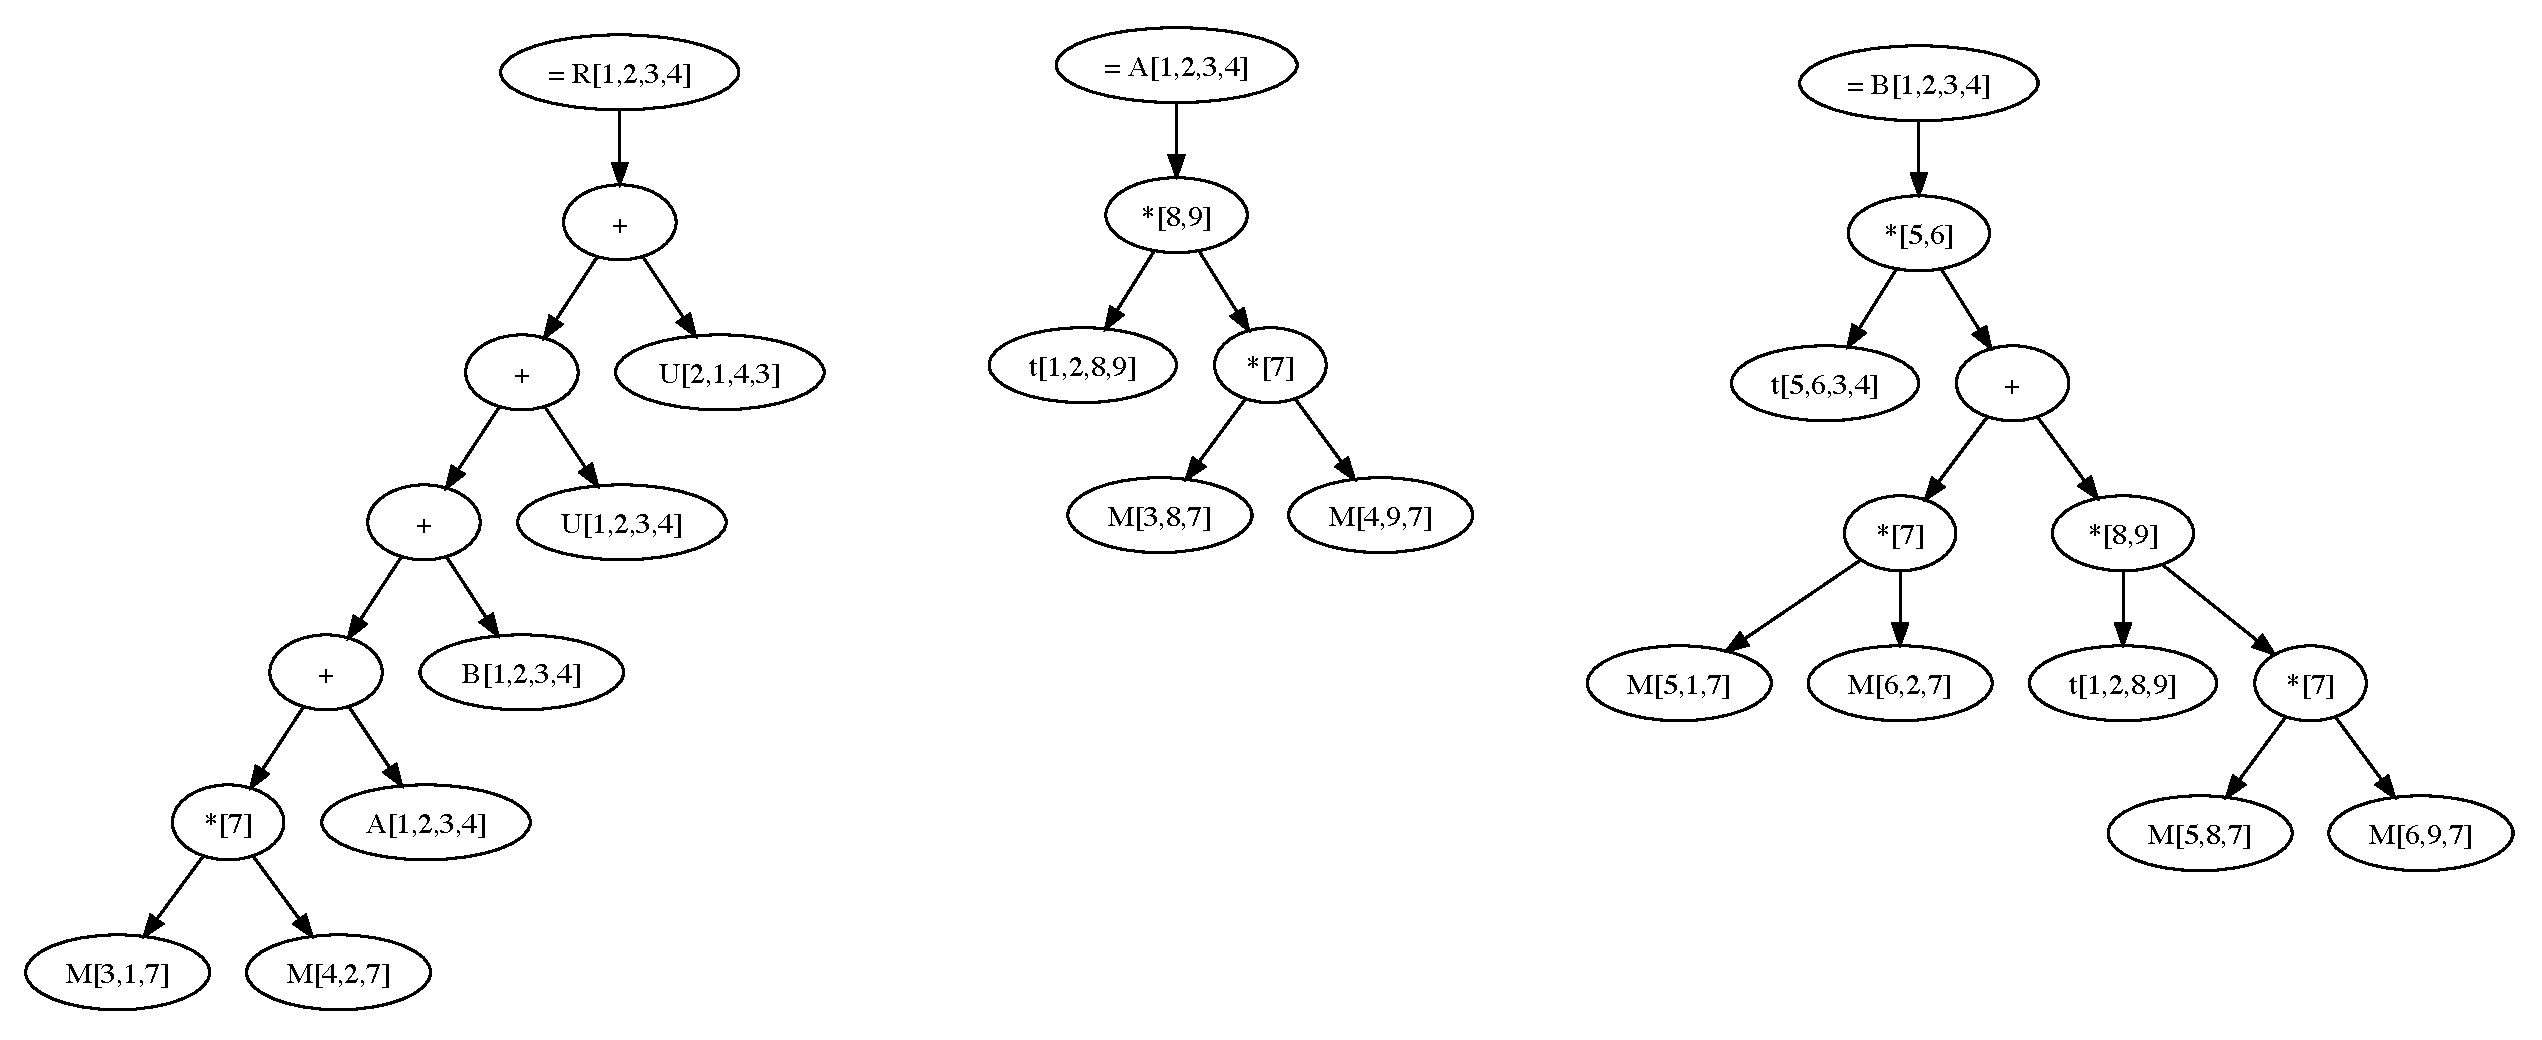
\includegraphics[width=0.9\textwidth]{dag.eps}
\caption{Initial expression tree parsed from \LaTeX{} source.  Execution order is from bottom to top, with the topmost node representing an output.  Index symbols have been converted to (lexically scoped) integers. Contractions are labeled with $*$ and a list of summation indices.  Named intermediate tensors are indicated with dummy, label nodes (= C[1,2]) etc.}
\label{f:dag}
\end{figure}

  Next, the nodes of the DAG are transformed into local operations by replacing the index
labels with local permutation indices.  % using a top-down tree traversal.
The new Sum, Diff, and Dot nodes contain permutation lists for finding the input dimension
corresponding to a given output dimension.
Named intermediates are also linked into their parent at this stage.

  The result will be a DAG of tensor operations,
\begin{verbatim}
struct net_tensor {
  network_ptr *location; // where / how is the tensor accessed
  struct tensor *A; // actual data, if local
};

struct tens_gen {
  int n; // dimension
  int *shape; // list of n integers
  (*gen)(float *row, int *); // function generating row of values
};

struct tens_dot {
  struct tens_op *A, *B;
  int n; // number of output dimensions
  int m; // number of contracted dimensions
  int *dA, *dB; // list of n indices to output from A and B
  int *cA, *cB; // list of m indices to contract from A and B
};

struct tens_op {
  enum TensOP type; // 1 = tensor constant, 2 = tens_gen, 3 = tens_dot
  union {
    struct net_tensor *const; // type = 1
    struct tens_gen *gen; // type = 2
    struct tens_dot *dot; // type = 3
  };
};
\end{verbatim}

  This DAG will be the target of algebraic optimization techniques aimed at reducing the total operation
count.

  The overall operation tree will then be a {\tt struct tens\_op}.  When that top-level
{\tt tens\_op}'s type is constant, the computation is finished.  Otherwise, the chain of references
forms a directed acyclic graph with lots of pending operations (leaves of type tens\_dot).

  The reference execution model will find a {\tt tens\_op} with type {\tt tens\_dot} and two
leaves of type {\tt tens\_gen} or {\tt tens\_const}.  It will then execute the contraction, producing
a {\tt struct tensor} in local memory.  Then two leaves will be submitted to garbage collection (decrement
refcount), and the completed {\tt tens\_dot} will be replaced with the new value.

  Eventually, we may augment the tree with information to minimize communication.

\subsection{ Reference Tensor Representation}

  Drawing from the representation in the {\em numpy} library
(\href{http://docs.scipy.org/doc/numpy/reference/arrays.html}{ndarrays} -- see C-struct access),
a tensor is composed of a header and a large data block.  The header contains the following information about accessing elements of the data block

\begin{itemize}
\item n -- the logical dimension of the array
\item shape -- a list of n integers, stating the length along each dimension
\item strides -- a list of n integers, stating the number of bytes to skip for
travel along each direction
\end{itemize}

  For example, an order 4 tensor with shape (4,5,2,7) would have
$4*5*2*7 = 280$ floats.  The general element A[i,j,k,l] would accessed like:

\begin{verbatim}float *A;
int strides[] = {5*2*7, 2*7, 7, 1};
float x = A + i*strides[0] + j*strides[1] + k*strides[2] + l*strides[3];
\end{verbatim}

  Tensor transposition can be accomplished just by changing the header information.
For example, to access old element [i,j,k,l] like [i,l,k,j], we need to swap dimensions 1 and 3.
The strides then change from (5*2*7, 2*7, 7, 1) to (5*2*7, 1, 7, 2*7).  In {\em numpy}, this
is done with the call {\tt A = transpose(A, (0,3,2,1))}.

\subsection{ Reference Contraction}

  The basic operation is contraction.  Contraction of a (3,2,4) tensor $\tens{A}$
and a (2,4,7) tensor $\tens{B}$ along the (2,4) axes would produce a (3,7)
tensor like so:

\begin{verbatim}float *C = malloc(sizeof(float)*3*7);

for(k=0; k<3; k++) { for(l=0; l<7; l++) {

for(i=0; i<2; i++) {
   for(j=0; j<4; j++) {
     C[k,l] += A[k,i,j]*B[i,j,l];
   }
}

}}
\end{verbatim}

  Of course the memory accesses are indexed as above.  Contraction should always be
replaced by BLAS dgemm operations where possible.
These are likely already implemented in GPU libraries like Magma.

  Also, it makes sense to check for performance gains by completing several multiplications
at once.  This can be made to fit in GPU memory by breaking tensors into sub-blocks.
The theano library may provide a means of testing and and producing such optimizations.

\section{ Requirements}

  A library will be constructed containing the following core functionality:
\begin{enumerate}
  \item Tensor contraction (single-machine memory to memory
  \item DAG operations to select most suitable available contraction operation and manage storage of intermediate results (deleting when no longer needed as a dependency of another calculation).
  \item Interprocessor communication of a tensor. \\
   This will likely include setting up a pipeline for efficient transfer of larger data structures.  Overlapping communication and execution would be nice, but is not required at this stage.
  \item Tensor storage / read from disk \\
  This functionality is needed for storage of intermediate results in case the available memory of a machine is exhausted.
  Does mmap offer better performance for storing large tensors in memory?
\item Checking sizes of intermediate results. \\
  Eventually, this information will be used to better organize the order of operations.
\end{enumerate}

  The demo will invoke this library to solve the small-molecule test problem.

  Because the calculation is expected to be memory-bound, each compute node will operate by spawning
sub-processes (fork or thread) to execute ready-to-go operations from the bottom of the graph until its memory is exhausted.  One simple implementation strategy is to use mpi to launch one task per node and have that task spawn threads.

  Experience gained from this preliminary implementation will inform later
decisions on scheduling operations.

\section{ Possible FOSS Tools}

\begin{itemize}
  \item OpenMPI, high-level communication primitives (some RDMA support).  Note that GPU-direct RDMA is supported for sizes less than 30kb. \\
  \href{https://computing.llnl.gov/tutorials/mpi/samples/C/mpi\_latency.c}{latency test},
  \href{https://www.pdc.kth.se/education/tutorials/summer-school/mpi-exercises/mpi-lab-3-bandwidth-latency-and-timings}{timings}
  \item Magma, a GPU accelerated linear algebra library: \href{http://icl.cs.utk.edu/magma/}{http://icl.cs.utk.edu/magma/}
  \item Theano: a python tensor operation optimization library: \href{http://deeplearning.net/software/theano/index.html}{Docs} \\
   This has a backend for producing compiled CUDA code to do tensor contractions (float32 only)
  \item TCE the original tensor contraction engine: \href{http://www.csc.lsu.edu/\%7Egb/TCE/}{http://www.csc.lsu.edu/$\sim$gb/TCE/} \\
   As far as I can tell, this spreads each single tensor contraction over all nodes - a serious design limitation that was exacerbated by a team size that grew large and drifted in different directions.
That method of parallelization only works for the paradigm of having few contraction operations.
We have lots of contractions and need to spread those operations across nodes.   
  \item GNU Sci. Lib, a general purpose linear algebra library: \href{http://www.gnu.org/software/gsl/}{http://www.gnu.org/software/gsl/}
  \item \href{http://web.cs.uh.edu/~openuh/}{OpenUH} (supporting preliminary subset of OpenACC - \href{http://www.clustermonkey.net/Parallel-Programming/an-open-compiler-for-openacc.html}{announcement})
  \item Network coordination of tensor locations and remaining contractions can be managed through etcd or similar.  This will need a simple update mechanism for informing the network of accepted and complete jobs.
\end{itemize}

\section{ Demo Problem}

  The problem that will be solved for the initial publication of this method will be to reproduce the
implementation of the density-fitted CCSD equations as implemented by Eugene DePrince in
the GPU module (\href{https://github.com/edeprince3/gpu\_dfcc/blob/master/ccsd.cu}{gpu\_dfcc})
for \href{http://www.psicode.org/release_notes.php}{Psi4}.  The equations are listed
in \href{http://pubs.acs.org/doi/abs/10.1021/ct400250u}{DePrince and Sherrill, JCTC 9(6):2687, 2013.}
and more detail on the GPU implementation is given in
\href{}{DePrince, Kennedy, Sumpter, and Sherrill, Mol. Phys. 112: 844, 2014}.

  The DAG of primitive tensor operations can be read directly
from a subset of the \LaTeX{} math syntax and/or built by automated methods.
For example, the \LaTeX{} source for the first few elements of the residual equation:
\begin{align}
R_{ij}^{ab} &= \sum_Q M_{ai}^Q M_{bj}^Q + A_{ij}^{ab} + B_{ij}^{ab} + U_{ij}^{ab} + U_{ji}^{ba} \\
A_{ij}^{ab} &= \sum_{cd} t_{ij}^{cd} \sum_Q M_{ac}^Q M_{bd}^Q \\
B_{ij}^{ab} &= \sum_{kl} t_{kl}^{ab} \left( \sum_Q M_{ki}^Q M_{lj}^Q
                 + \sum_{cd} t_{ij}^{cd} \sum_Q M_{kc}^Q M_{ld}^Q \right)
\end{align}
was parsed into the expression tree in Fig.~\ref{f:dag}.  Here, $U_{ij}^{ab}$ is used to stand
for $\frac{1}{2}C_{ij}^{ab} + C_{ji}^{ab} + D_{ij}^{ab} + E_{ij}^{ab} + G_{ij}^{ab}$.

  It should be noted at the outset that the tensor names are non-unique without also giving
example indices.  This is because the tensor, $F \in \mathcal T_{o,v,o,v}$, for example,
can be written as the $ov \times ov$ matrix,
\begin{equation}
\begin{bmatrix}
\text{Fij} & \text{Fia} \\ \text{Fai} & \text{Fab}
\end{bmatrix}
.
\end{equation}
Most of the expressions in the paper related to one of the sub-blocks of a tensor
rather than the complete tensor.  This is acutely the case for $M$
($B_{\circ}^Q$ in the references).
The code again uses 4 different matrices,
\begin{equation}
\begin{bmatrix}
\text{Qoo}^Q & \text{Qov}^Q \\ \text{transpose}(\text{Qov})^Q =\text{Qvo}^Q & \text{Qvv}^Q
\end{bmatrix}
.
\end{equation}

\begin{figure}
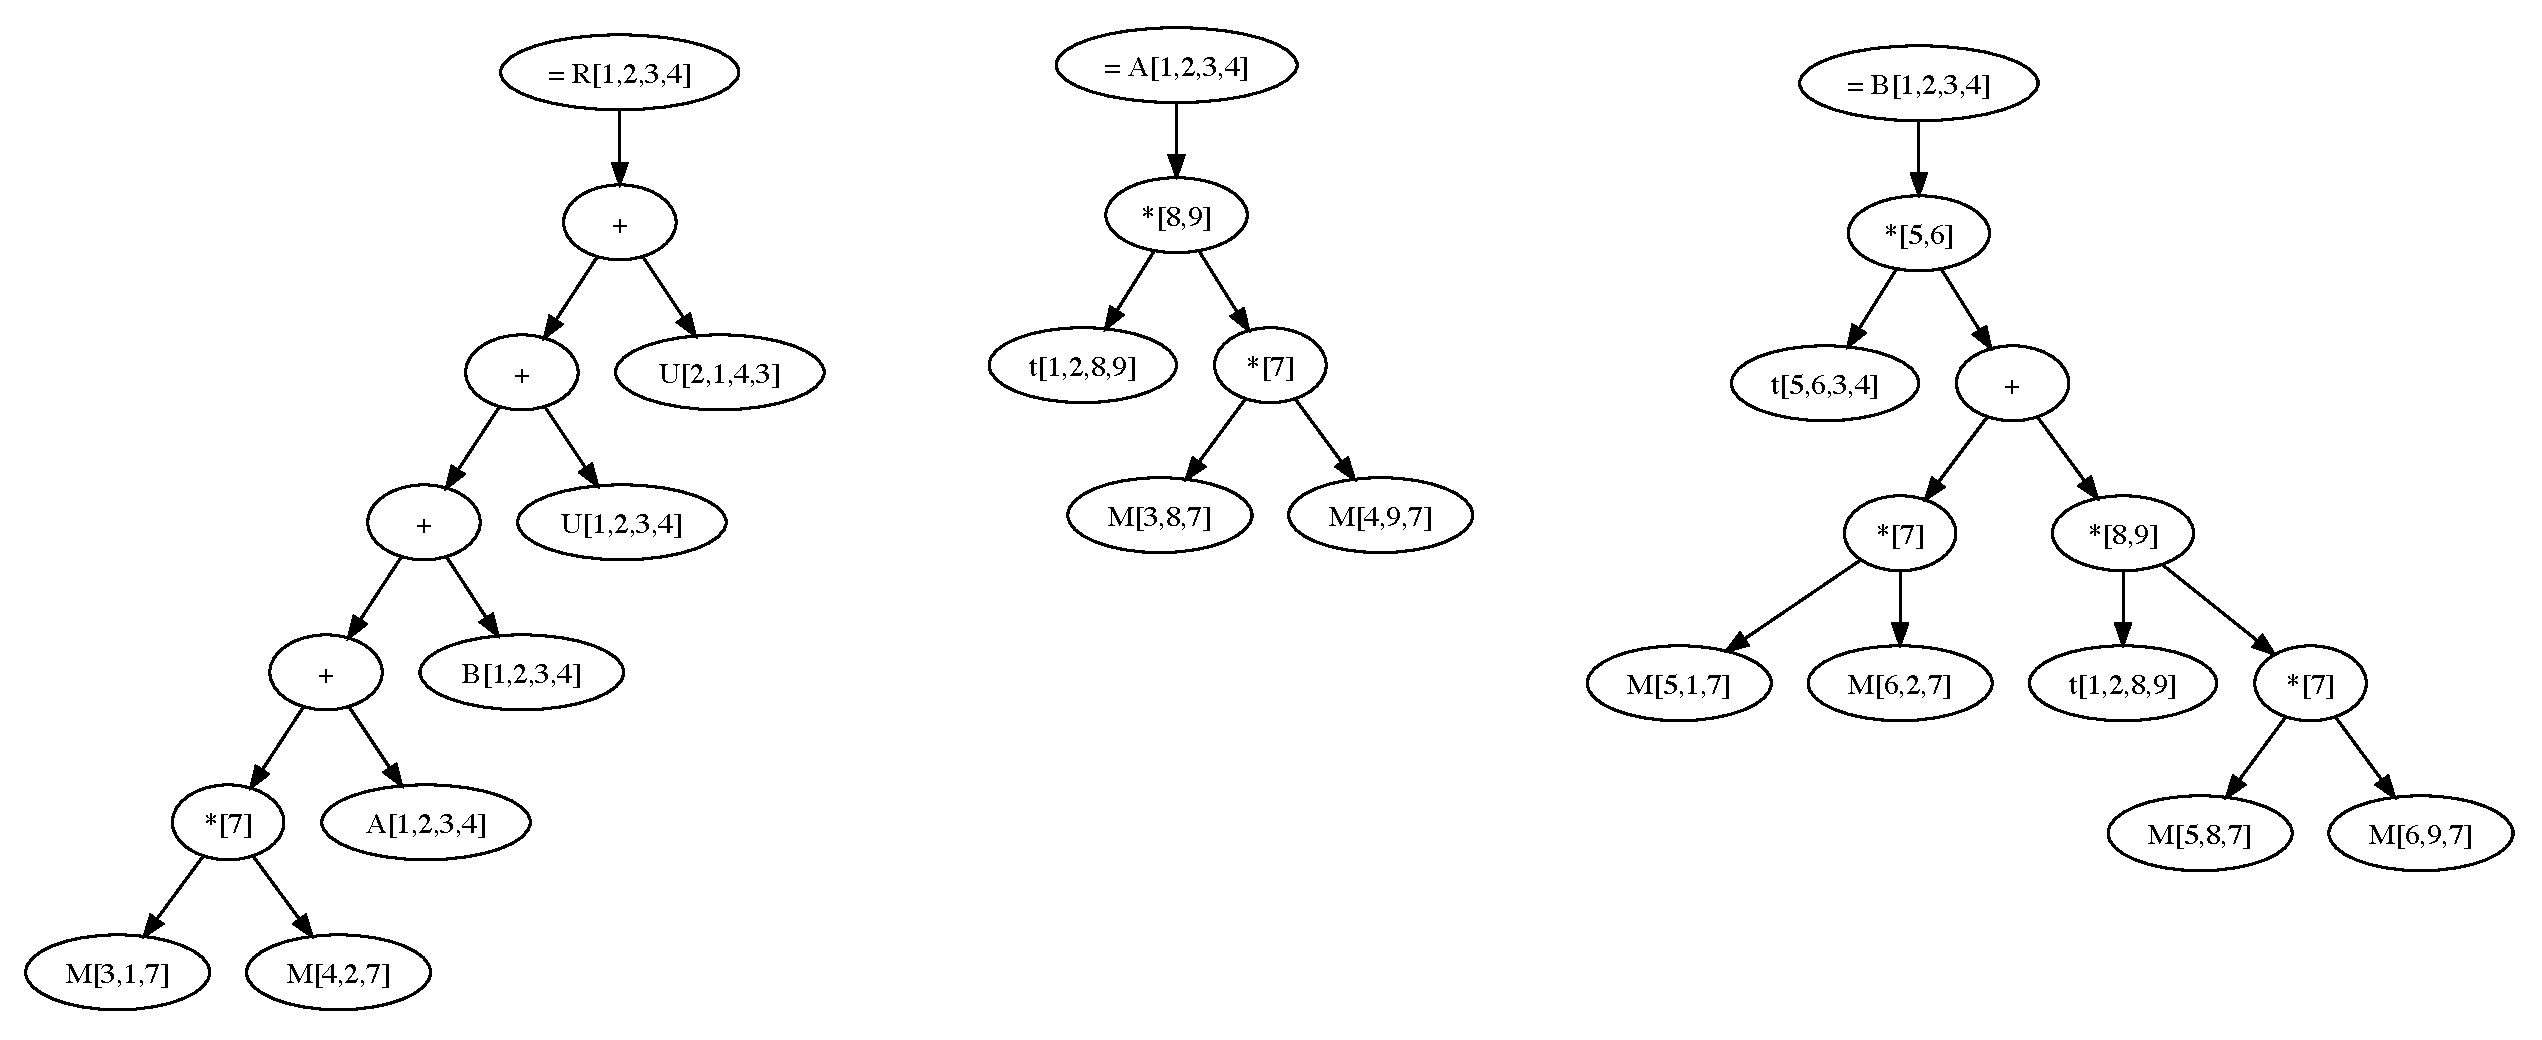
\includegraphics[width=0.9\textwidth]{dag.eps}
\caption{Initial expression tree parsed from \LaTeX{} source.  Execution order is from bottom to top, with the topmost node representing an output.  Index symbols have been converted to (lexically scoped) integers. Contractions are labeled with $*$ and a list of summation indices.  Named intermediate tensors are indicated with dummy, label nodes (= C[1,2]) etc.}
\label{f:dag}
\end{figure}

  Next, the nodes of the DAG are transformed into local operations by replacing the index
labels with local permutation indices.  % using a top-down tree traversal.
The new Sum, Diff, and Dot nodes contain permutation lists for finding the input dimension
corresponding to a given output dimension.
Named intermediates are also linked into their parent at this stage.

  The hand-coded implementation of the residual calculation ($R_{ij}^{ab}$) is
done in {\tt pthreadCCResidual}:1066.  This routine is called by each of at least 2 pthreads.
Thread 0 executes the GPU portion, assigning all available GPUs to compute $A_{ij}^{ab}$, which has
the largest matrix multiplication to carry out.  Its task is broken into tiles that fit
into the GPU memory.  The sizes of the tensors are given by malloc statements on lines
991--1026.

  Other threads are used in a gang to compute the rest of the
contributions to the residual {\em via} {\tt \#pragma omp parallel for}.  As I understand
OMP scheduling, the {\tt parallel for} spawns its own threads, so only 1 thread should
really be executing the pragma (otherwise work is duplicated).  This computation
starts by assembling $\tfrac{1}{2}C_{ij}^{ab} + C_{ji}^{ab}$ into a temp space,
$\text{tempt}$, where
\begin{equation}
C_{ij}^{ab} = -\sum_{kc} t_{kj}^{bc} \left[
\sum_Q M_{ki}^Q M_{ac}^Q - \frac{1}{2} \sum_{ld} t_{li}^{ad} (\sum_Q M_{kd}^Q M_{lc}^Q)
\right]
\end{equation}
is computed from the starting matrices, $M = \text{Qov}$, and the doubles amplitudes,
$t_{ij}^{ab} = \text{tb}$, via the following steps (on lines 1114--1255):
\begin{align}
\text{Qov} &\in \mathcal T_{o,v,n_Q} \\
\text{Qoo} &\in \mathcal T_{o,o,n_Q} \\
\text{Qvv} &\in \mathcal T_{n_Q,v,v} \\
\text{integrals} &= \text{Qov} \cdot \text{Qov}^T  \in \mathcal T_{o,v,o,v} \\
\text{tempt}[aild] \in \mathcal T_{vovo} &= \text{tb}[adli] \in \mathcal T_{v,v,o,o} \\
\text{tempv}[kcld] \in \mathcal T_{ovov} &= \text{integrals}[kdlc] \in \mathcal T_{o,v,o,v} \\
\text{integrals} &= \frac{1}{2} \sum_{kc} \text{tempt}[aild] \text{tempv}[kcld] \quad \text{(tiled)} \\
\text{tempv} &= \text{Qvv}^T \cdot \text{Qoo}^T \\
\text{integrals} &= \text{integrals} + \text{tempv} \\
\text{tempt}[bjkc] &= \text{tb}[bckj] \\
\text{tempv}[bjai] &= -\sum_{kc} \text{integrals}[acki] \text{tempt}[bckj] \quad \text{(tiled)} \\
\text{tempt}[abij] &= \frac{1}{2} \text{tempv}[bjai] + \text{tempv}[biaj]
.
\end{align}
This symmetrized sum of $C$ is then added to the residual and stored on disk.
The calculation then takes a break and does the singles residual,
\begin{equation}
R_i^a = F_{ai} + \sum_{dQ} \sum_{kc} u_{ki}^{cd} M_{kc}^Q M_{ad}^Q
  - \sum_{klc} u_{kl}^{ac} \sum_Q M_{ki}^Q M_{lc}^Q
  + \sum_{kc} F_{kc} u_{ik}^{ac}
  ,
\end{equation}
from which $u_{ij}^{ab}$ (in {\tt tempt}) is a by-product (which is recomputed later anyway?).

  The doubles calculation picks back up on line 1360, with $D$, $E$, $G$, and $B$.
The $\sum_Q M^Q_{kd}M^Q_{lc}$ part is shared between $E$ and $G$ using the
`integrals' buffer.
Each time it reads the last residual from the disk,
adds the new contribution, and stores the result.

  Finally $A$ is added into the residual ({\tt useVabcd1}) after all threads complete and control returns to
{\tt CCResidual:1704}.  If the cpu calculations finish first, {\tt FinishVabcd1} aids the gpu in completing the
calculation of $A$.  It is unclear what part of the code calls {\tt T1Fock} to compute $F_{ia}$ and $F_{ai}$,
but a comment notes that it is recomputed at each iteration -- so it's likely the DIIS driver that also calls {\tt CCResidual}.

  Many of these calculations also use matrix tiling, illustrated by Fig.~2 of the Mol. Phys. article.
In particular, the tiling of the $A$ tensor will need to be considered to minimize idle time.
Basically, the contraction is divided into smaller sub-blocks of the output.  The picture is like Strassen's matrix
multiplication algorithm, where the output is divided into $2\times 2$ blocks, $\begin{bmatrix}a_{00} & a_{01} \\ a_{10} & a_{11} \end{bmatrix}$.
\begin{align}
A &\gets B \cdot C \\
& \to A \gets \text{combine}(B[:n/2] \cdot C[:,:m/2], B[:n/2] \cdot C[:,m/2:], \ldots)
\end{align}
This can be put into the operation DAG by introducing {\tt combine} and {\tt split} operations.
A contraction over a tensor with large dimension sizes can be replaced by a series of
contractions sandwiched between these combine and split operations.

  The $A$ tensor also has symmetry which allows it to be stored as 2
compressed, lower-diagonal matrices.
One is symmetric and the other anti-symmetric with respect to
interchanging either $i\leftrightarrow j$ or $a\leftrightarrow b$
(equations 31-37 of the JCTC paper).

  The memory is accessed using the {\tt Position} function,
called wherever tensor symmetry is used.
See especially the lines 254--310 where $A$ is added to the
$\mathcal T_{v,v,o,o}$ residual (exactly the shape of the {\tt t2}
matrix, confusingly called {\tt tb} in the code).
Symmetry will require replacing the Dot operation in the task DAG
with a symmetry-aware contraction operation, and adding
a special flag to the $A$ tensor to note its symmetric storage type.


\end{document}
